%!TEX root = thesis.tex
\chapter{Demonstrator}
\label{sec:demo}

To demonstrate the work described in the previous chapters in a real world
application, a ball on plate system is presented in the following sections.
The demonstrator tries to balance a ball by tracking its position and
adjusting the angle of the underlying plate, thus allowing to compensate
external impacts and keeping the ball in the center. Therefore, the plate
itself is mounted on top of a Stewart platform and has a resistive touchscreen
attached to it. While the Stewart platform offers the ability to rotate the
plate around arbitrary axes, the touchscreen provides precise and low latency
positioning information of the ball.

The control of the platform is implemented by a \ac{PAC} based on the previous
considerations, including analog I/O, low latency data paths and control
loops, as well as self-adaptive capabilities. The different components of the
system are described in detail in the following sections. These include the
kinematics of the Stewart platform, the touchscreen interface and control
algorithms for balancing the ball.

\section{Stewart Platform}
The Stewart platform was introduced by D. Stewart in 1965 \citep{Ste65} and
gained popular resarch interest in robotics \citep{Szu13}, concerning
kinematics, dynamics or work space estimations. However, outside the
scientific community the Stewart platform was not widely adopted and most
designs are constrained to applications requiring \ac{6DoF}, for instance
flight simulators or \ac{CNC} machining centers. Although a Stewart platform
provides many potential advantages , sophisticated synthesis and simulation
tools are missing \citep{Ji96}. Against the background of increasing
computational capabilities and more efficient \ac{CAD} tools, this situation
might change in the future. In the scope of this thesis, the Stewart platform
promises to be a sophisticated development platform, involving computationally
expensive calculations for its kinematics and need for additional I/O
capabilities.

The following sections introduce the architecture of the Stewart platform in
general and the variant used in this thesis, specifying the used notation and
solving the inverse kinematics problem.

\subsection{Architecture}
While Stewart introduced the general idea of a Stewart platform in his work in
1965 \citep{Ste65}, a strict definition is missing in the literature. The only
commonality is the characterization as a parallel manipulator \citep{Szu13}
consisting out of a bottom base and an upper platform. Compared to a serial
manipulator, it consists out of multiple serial chains controlled
simultaneously and connected to a single end-effector. While this design
provides unique benefits like high accuracy, better load-to-weight ratios and
improved rigidity, it limits the available work space and causes highly
nonlinear behavior.

%\begin{figure}
%	\centering
%	\begin{subfigure}{0.3\textwidth}
%		\centering
%		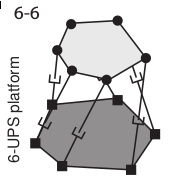
\includegraphics[width=\textwidth]{../figures/stewart_architectures_c}
%		\caption{6-UPS}
%		\label{fig:stewart_architectures_a}
%	\end{subfigure}
%	\begin{subfigure}{0.3\textwidth}
%		\centering
%		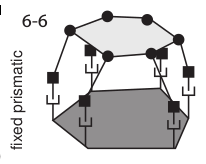
\includegraphics[width=\textwidth]{../figures/stewart_architectures_d}
%		\caption{Fixed prismatic}
%		\label{fig:stewart_architectures_b}
%	\end{subfigure}
%	\begin{subfigure}{0.3\textwidth}
%		\centering
%		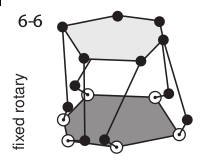
\includegraphics[width=\textwidth]{../figures/stewart_architectures_e}
%		\caption{Fixed rotary}
%		\label{fig:stewart_architectures_c}
%	\end{subfigure}
%	\caption{Different variants of Stewart platforms \citep[adopted from][]{Szu13}}
%	\label{fig:stewart_architectures}
%\end{figure}
The different variant of a Stewart platform vary in the type of the
connections and actuators, as well as their spacial configuration, i.e. the
positioning of the different connections. The most common realization utilizes
six prismatic actuator, for example hydraulic pistons or linear motors. It is
often referred to as Hexapod and associated with the term Stewart platform,
not least because of its similarity to the original design proposed by
Stewart. Other architectures utilize fixed prismatic or rotary actuators as to
vary the length of the six legs. All of these variants have its unique
benefits and drawbacks. Since the actuators in the latter design can be
realizing as commonly available servo motors, it gained popularity, especially
for low-cost designs and first prototypes. Therefore, this thesis focuses on a
servo-based architecture as shown in figure
\ref{fig:stewart}. The mechanical design and construction was not done in this
thesis, but adopted from a previous work.
\begin{figure}
	\centering
	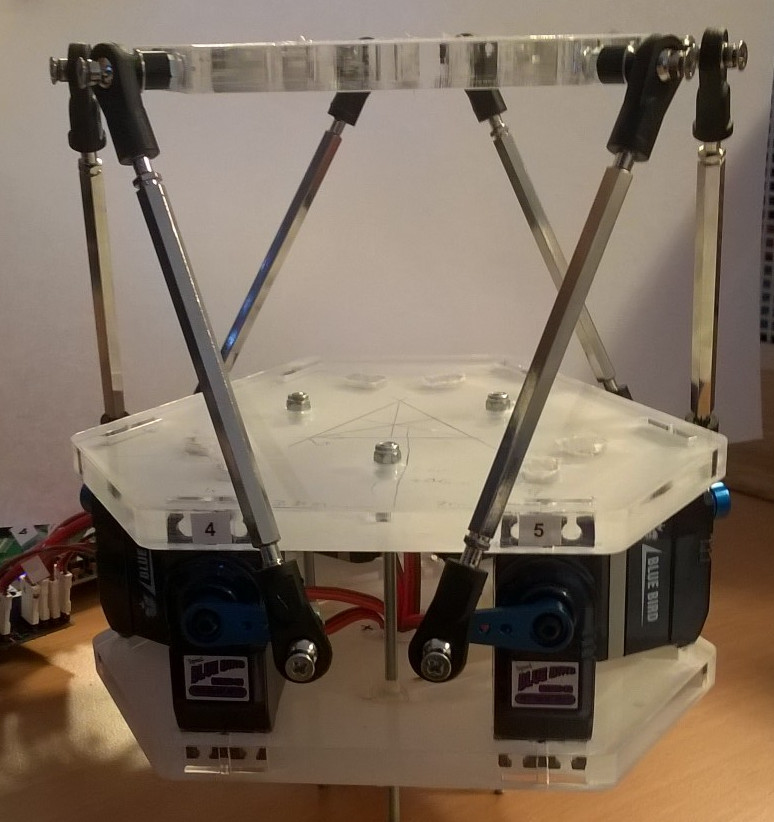
\includegraphics[width=6cm]{../figures/stewart}
	\caption{Construction of the Stewart platform prototype}
	\label{fig:stewart}
\end{figure}

\subsection{Construction and Notation}
This section introduces the basic notations, coordinate systems and dimensions
of the Steward platform used in this thesis. Consider figure
\ref{fig:stewart_notation}, showing different views annotated with relevant
notations.
\begin{figure}
	\centering
	\begin{subfigure}{0.49\textwidth}
		\centering
		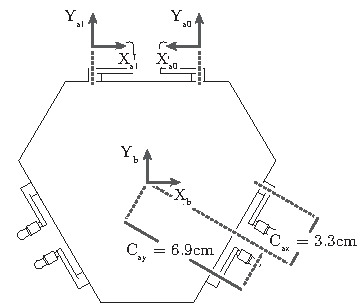
\includegraphics{../figures/stewart_base}
		\caption{Top view of base}
		\label{fig:stewart_base}
	\end{subfigure}
	\begin{subfigure}{0.49\textwidth}
		\centering
		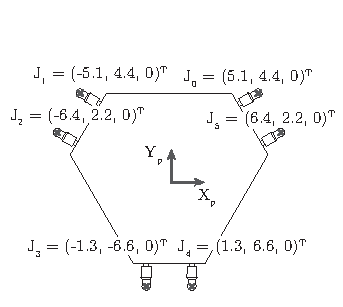
\includegraphics{../figures/stewart_platform}
		\caption{Top view of platform}
		\label{fig:stewart_platform}
	\end{subfigure}
	\par\bigskip
	\begin{subfigure}{0.49\textwidth}
		\centering
		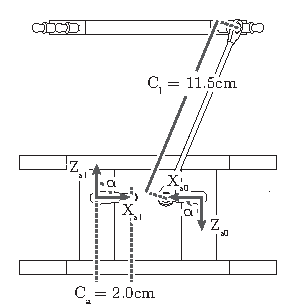
\includegraphics{../figures/stewart_side}
		\caption{Side view}
		\label{fig:stewart_side}
	\end{subfigure}
	\caption{Notations for the Stewart platform}
	\label{fig:stewart_notation}
\end{figure}

As already described previously, the system consists out of a lower base and
an upper platform, connected by six legs. For both, the base and platform, a
particular coordinate system is introduced as shown in figures
\ref{fig:stewart_base} and \ref{fig:stewart_platform}. While origin of the
base coordinate system $B$ is located in the center of the base and at the
same height as the shaft of the servos, the origin of platform's coordinate
system $P$ is located exactly above at the height of the platform joints
$J_i$. With regard to the platform's coordinate system, the coordinates of the
six joints are annotated in figure \ref{fig:stewart_platform}.

Additionally, each servo specifies its own coordinate system $S_i$, located at
the intersection point of the servo's shaft and the servo's joint position.
Thereby, the y axis points away from the base and the x axis to servo's joint
in neutral position. Resulting from these two axes, the z axis points up or
down, depending of the servo, i.e. for even servos it points down and for odd
servos it point up. Figure \ref{fig:stewart_side} illustrates the servo
coordinate systems again and showing the angle $\alpha$ of the servo arm. The
different coordinate systems for even and odd servos allow to handle all
servos analogously and respects the physical configuration of the servo arms.

Calculating the inverse kinematics of the platform requires to transform the
joints of the platform to the corresponding servo coordinate system. This is
done in two steps, by transforming them to $B$, and finally to $S_i$. While
the transformation to the base coordinate system $B$ is trivial, by simply
adding an offset $C_h$ to the z coordinate, transforming the resulting point
to the servo coordinate system $S_i$ requires more sophisticated calculations,
including rotation and scaling. At first, the base coordinate system is
rotated to match the y axis of the appropriate servo coordinate system,
followed by mirroring the x and z axis to fit the desired orientations.
Finally, the origin is translated to match the servo positions by adding and
subtracting $C_{sx}$ and $C_{sy}$ to the x and y coordinates, respectively.

\subsection{Inverse Kinematics}
Taking the basic notations of the previous section as a basis, the inverse
kinematic calculates the required servo positions for a desired angle of the
platform. Unlike for serial manipulators, the inverse kinematics of a Stewart
platform has a unique analytic solution, while the forward kinematics problem
is highly nonlinear and requires iterative approaches. However, the low-cost
variant utilizing rotary instead of linear actuators introduces additional
calculations to calculate the required angles from the desired leg lengths.

Assuming, that the desired angle of the platform is given by a rotation axis
$r$ and a rotation angle $r_a$, equation \ref{eq:platform_rot} shows the
calculation of the required platform joint's positions.
\begin{equation}
J'_i = 
\begin{pmatrix}
\left[\left(1 - \cos(r_a)\right) r_x r_x + \cos(r_a)\right] J_ix + \left[\left(1 - \cos(r_a)\right) r_x r_y\right] J_iy\\
\left[\left(1 - \cos(r_a)\right) r_x r_y\right] J_ix + \left[\left(1 - \cos(r_a)\right) r_y r_y + \cos(r_a)\right] J_iy\\
\left[-r_y \sin(r_a)\right] J_ix + \left[r_x \sin(r_a)\right] J_iy\\
\end{pmatrix}
\label{eq:platform_rot}
\end{equation}
Transforming these position to the appropriate servo coordinate systems as
described in the previous section allows to calculate the distance between the
servo joint and the platform joint. While for a linear actuator this would be
the solution, rotary actuators can not vary the length of the legs directly.
Therefore, the angle $\alpha$ must be adjusted in a way, that the distance
between its joint and the platform joint is equal to the fixed leg length
$C_l$. While there exist an analytic solution for this problem, it includes
terms of higher degree and complex operations like $\arctan$ and square roots.
Therefore, an iterative approach was chosen to find the appropriate angle.
More details on the concrete implementation of this iterative approach will be
covered in the implementation section.

\section{Touchscreen}
To track the ball's position on the plate, a resistive touchscreen is mounted
on top of the plate and touched by the ball. Compared to, for example camera
based tracking techniques, a touchscreen provides low latency data independent
from external influences like lighting conditions or camera movements.
Furthermore, it requires less computational effort, as well as a more compact
setup.

The following subsections introduce briefly the fundamental principles of the
resistive touchscreen technology and covers the use in the prototype.

\subsection{Resistive Touchscreen Technology}
An analog resistive touchscreen consists out a glass substrate and a flexible
film, both coated with a conductor \ac{ITO} \citep{Wal12}, as shown in figure
\ref{fig:touch_build}.
\begin{figure}
	\centering
	\begin{subfigure}{0.49\textwidth}
		\centering
		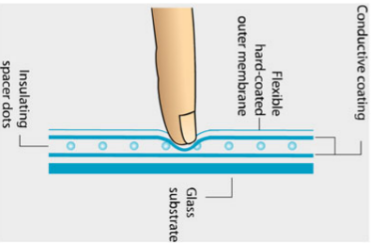
\includegraphics{../figures/touch_build}
		\caption{Construction of resistive touchscreen}
		\label{fig:touch_build}
	\end{subfigure}
	\begin{subfigure}{0.49\textwidth}
		\centering
		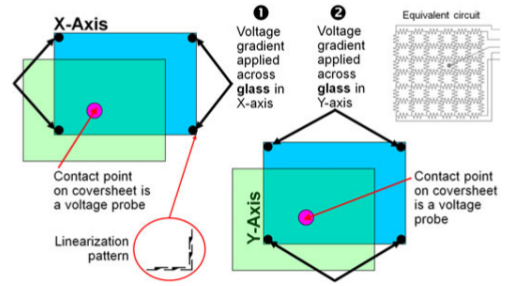
\includegraphics{../figures/touch_five}
		\caption{Five-wire touchscreen}
		\label{fig:touch_five}
	\end{subfigure}
	\caption{Analog resistive touchscreen technology \citep[adapted from][]{Wal12}}
	\label{fig:touch}
\end{figure}
The two conductive surfaces are facing each other and
are separated by insulating spacer dots \citep{Wal12}. When a voltage is
applied across the surfaces and the flexible film is pressed down, the two
surfaces make electrical contact, resulting in a voltage divider created by
the resistance of the \ac{ITO}. Measuring the ratio of the different voltages
allows to calculate the touch position.

Basically, there exist three major variants of resistive touchscreens, namely
four-wire, five-wire and eight-wire touchscreens, differing in the number of
connections to the sensor \citep{Wal12}. For the demonstrator, a five-wire
touchscreen was used as shown in figure \ref{fig:touch_five}, due to its
increased durability and sustainability. The X and Y voltages are applied to
the four corners of the lower glass, while the upper film is used only as a
contact point to measure the voltage at the touch position (wiper). To
determine, for example, the X position, a voltage is applied to the two left
corners, while two right corners are connected to ground.

\subsection{Interfacing the Touchscreen}
To interface the touchscreen, voltage needs to be applied to different corners
of the touchscreen, while all other ones needs to be connected to ground.
Therefore, regular digital I/O are sufficient, setting their output to 1 or 0,
respectively. To measure the voltage at the touch point through the viper, an
\ac{ADC} with suitable input ranges is required. To eliminate noise caused by
an unstable voltage source, the \ac{ADC} should be connected in a differential
fashion to the wiper and the supply voltage. This improves the reliability and
minimizes the effects of voltage fluctuations \citep{OOD00}.

In this work, the pre-assembled evaluation module ADS7845EVM \citep{ADS06} was
used. While the ZedBoard provides both digital I/O and an on-chip \ac{ADC}
which could be utilized to interface a touchscreen, additional circuits would
be required to meet the \ac{ADC}'s input requirements. Since circuit design is
not target of this thesis, a pre-assembled evaluation module was chosen. It
provides an appropriate connector for the touchscreen and interfaces with the
\ac{FPGA} via the \ac{SPI} interface as shown in figure \ref{fig:touch_spi}.
\begin{figure}
	\centering
	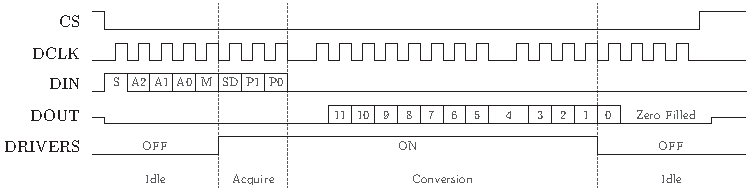
\includegraphics{../figures/touch_spi}
	\caption{\acs{SPI} interface of the ADS7845 touch controller \citep[adapted from][]{ADST06}}
	\label{fig:touch_spi}
\end{figure}
A single conversion is done in 24 clock cycles with a period of
$\SI{400}{\nano\second}$ by sending eight configuration bits to the controller
and receiving the converted voltage at the touch position as a 12 bit integer.
The configuration bits send in the first byte include the channel selection
\emph{A2} - \emph{A0}, i.e. the x and y directions, mode selections and power
down options. The \emph{SD} bit selects between single-ended and differential
mode, \emph{M} selects between eight and twelve bit conversion and \emph{P1} -
\emph{P0} control the power down between conversions. After the control byte
is send, the controller enters the conversion mode and performs the analog-to-
digital conversion in the next twelve clock cycles. In the 13th clock cycle
the last bit is transferred, followed by three zero bits to complete the last
byte. Therefore, 48 clock cycles are necessary to read the x and y coordinate
of the touch position, i.e. around $\SI{20}{\micro\second}$.

To connect the controller evaluation module to the ZedBoard, regular digital
I/Os are required for the serial interface, as well as a $\SI{3.3}{\volt}$
voltage supply, provided by one of the \ac{Pmod} connectors.

\section{Control Algorithm}

\section{Implementation}
While the previous sections covered the fundamentals for the demonstrator and
addressed the main problem definitions, this section focuses on the
implementation of the different components. Consider figure
\ref{fig:demo_structure}, illustrating the overall structure of the system.
\begin{figure}
	\centering
	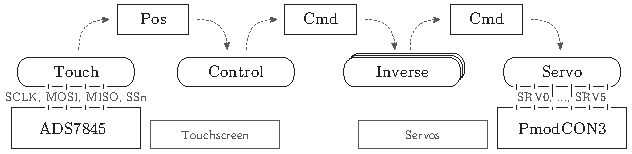
\includegraphics{../figures/demo_structure}
	\caption{Overall structure of the demonstrator}
	\label{fig:demo_structure}
\end{figure}
It consists out of four types of ReconOS threads representing the control loop
of the ball on plate application, which are synchronized and connected via
mailboxes to each other. The \emph{Touch} thread interfaces with the external
ADS7845 touch controller by implementing an \ac{SPI} master and provides the
positioning information to the \emph{Control} thread. That implements the
\ac{PID} controller and passes the manipulated variable, i.e. the rotation of
the platform, to the \emph{Inverse} thread. Since the inverse kinematic
constitutes the most computational intensive task and must be performed for
each of the six legs, it is parallelized in multiple threads, each one
calculating a single servo position. Therefore, one to six \emph{Inverse}
threads might be instantiated.

While the \emph{Touch} and \emph{Servo} threads must be implemented as
hardware threads, allowing them to interface with the I/O ports of the FPGA,
the remaining partitioning can be performed arbitrarily. Both the control and
inverse kinematics implementations are available for hardware synthesis, as
well as for software compilation.

\paragraph{Touch} As described in the previous section on the touchscreen
technology, an ADS7845EVM evaluation module is utilized in this work. The
\emph{Touch} thread implements the \ac{SPI} master according the ADS7845's
specifications and provides positioning information to the other threads. The
\ac{SPI} controller generates the required $\SI{2.5}{\mega\hertz}$ clock and
implements shift registers for both sending and receiving data.

\paragraph{Servo} The servos of the Stewart platform are controlled by a
\ac{PWM} signal, specifying the angle of the mounted arm. The thread receives
the required angle encoded as an integer together with a servo id via the
incoming mailbox and generates an appropriate \ac{PWM} signal. According the
servo's specification, the pulse must have a width of $\SI{1}{\milli\second}$
to $\SI{2}{\milli\second}$ and a period of $\SI{10}{\milli\second}$ to
$\SI{22}{\milli\second}$, resulting in the minimal or maximal angle,
respectively. Additionally to the control signal, the servos require an
external power supply, since the ZedBoard is not capable of providing
sufficient power. Therefore, the PmodCON3 modules provide a dedicated power
input and connect the control signals directly to the servo.

\paragraph{Inverse} The computationally most demanding component of the
application is the solution of the Stewart platform's inverse kinematics
problem. Therefore, it provides  potential for a speedup by a hardware
implementation. While the inverse kinematics problem itself was already
discussed in a previous section, this paragraph focuses on its implementation.
Since it contains many arithmetic operations including fixed point
calculations, it fits perfectly for an implementation in Vivado HLS. However,
while the tool includes a math library, it is not able to synthesize sine and
cosine functions. Therefore, an array synthesized into block \ac{RAM} is
precalculated and used as a lookup-table. The fixed point data type
\lstinline{ap_fixed<22,10>} is used for all calculations, providing sufficient
accuracy for this application. The resulting angle is encoded as an integer of
11 bits, resulting in a precision of $\SI{0.1}{\degree}$. As already
mentioned, the servo angle is calculated out of the leg length by a linear
search over all possible angles. Although an analytical solution could be
formulated, it requires square roots, high potencies and tangent functions,
making it harder to implement on an FPGA.

\section{Self-Awareness}
While the system described so far implements the basic functionality of the
ball-on-plate demonstrator, this section focuses on self-adaption strategies
by extending the demonstrator with a framework to gather self-aware properties
and introducing basic self-expression capabilities to optimize the power
consumption.

As stated in the background chapter, self-aware systems require knowledge of
themselves by acquiring so-called self-*properties, for example by capturing
sensor data or maintaining performance counters. This self-aware knowledge can
then be processed by a self-expression engine to modify the system's behavior
and meet specified requirements. Consider figure \ref{fig:demo_selfaware},
presenting an extended structure of the demonstrator, implementing the concept
of a self-aware system.
\begin{figure}
	\centering
	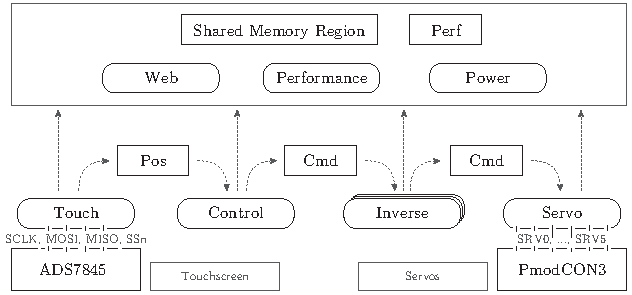
\includegraphics{../figures/demo_selfaware}
	\caption{Extended structure of the demonstrator}
	\label{fig:demo_selfaware}
\end{figure}
A globally accessible shared memory region allows to collect various types of
self-aware properties from different sources. For example, the \emph{Power}
thread acquires sensor data to measure the system's power consumption or the
\emph{Inverse} threads maintains a performance counter. All this data is then
utilized by the \emph{Self} thread, implementing a self-expression engine
consisting out of rules, adjusting parameters of the system. Furthermore, to
monitor the insights of the system, the \emph{Web} threads provides access to
several of the self-properties and parameters via an interactive web
interface.

The following subsections explain the different self-properties and how they
are acquired, as well as the adaptions strategies and controlled parameters of
the system. The following sections introduce the different properties in more
detail.

\subsection{Self-Properties}

The self-properties are acquired by the threads of the system and stored in
the globally accessible shared memory region. While the acquiring of the
properties is typically performed in parallel to the regular processing, the
additional memory accesses introduces an overhead and might effects the
overall system's performance. However, since the shared memory is not utilized
in the system so far, the overhead can be neglected. For software threads a
single word access is, obviously, not performance critical and a hardware
thread requires less than 10 clock cycles for an access via the memory
subsystem. It does not need to block until the word is written to the system
memory, but can proceed after the request is written to the \ac{MEMIF}
\ac{FIFO}.

To demonstrate self-adaptive capabilities of the system, the power
consumption, the ball's position on the plate and performance measures of the
computational intensive inverse kinematics solver are acquired and processed
by the self-expression engine.

\subsubsection{Power Consumption}
The power consumption of the system is affected by many components, ranging
from different threads through the entire the Zynq \ac{SoC} to external
devices like the touch controller. Therefore, a fine-grained measurement of
the different component's power consumption would be desirable, allow a more
sophisticated control of power requirements.

While more advanced boards include power measurement capabilities through
dedicated components connected to the FPGA, the ZedBoard only features a
$\SI{10}{\milli\ohm}$ current sense resistor in series with the
$\SI{12}{\volt}$ input power supply \citep{ZedBoard}. Measuring the voltage
drop at that resistor allows to calculate the current flowing into the board,
and, consequently, the power consumption of the system like in equation
\ref{eq:power}. $V_i$ represents the input voltage from the power supply, i.e.
$\SI{12}{\volt}$, and $V_s$ the measured voltage drop at the shunt resistor.
\begin{equation}
P = V_i I = V_i \frac{V_s}{\SI{10}{\milli\ohm}}
\label{eq:power}
\end{equation}
Since the resistor is placed on the high side, i.e. before any load, it has a
common mode voltage of around $\SI{12}{\volt}$, far exceeding the capabilities
of the on-chip \ac{ADC}. Therefore, the dedicated current sensing amplifier
\todo{LTC4151} is used to measure voltage drop $V_s$. It integrates an
instrumentation amplifier with an appropriate \ac{ADC} and reports data
through the \ac{I2C} interface, connected the Zynq's dedicated \ac{I2C}
controller. This allows to poll the \todo{LTC4151} from a regular software
thread and make it available via the self-properties memory region. Since this
region is globally accessible, both hardware and software threads can access
this data.

Based on the the overall power consumption of the board, different methods for
a more fine-grained measurement can be discussed. Directly measuring the power
consumption of single threads is not feasible, but suitable models could be
applied to estimate the power distribution across the chip. Different works
have dealt with the problem of simulating the power consumption of \acp{FPGA}
\citep{DeTu05,JeCa11} and commercial tools like Xilinx XPower are available to
estimate the resulting drawn. However, the effective switching activity
heavily depends on the input at runtime. Furthermore, external components are
not included in the simulation results and software threads running on an
operating system are heavily dynamic and unpredictable. Especially in case of
self-adaptive systems acquiring parameters at runtime, long running
simulations are not applicable. Therefore, learning strategies observing the
state of the system and its work load seem to be more suitable for power
estimation at runtime. While turning on and off threads or disabling external
components temporarily, the system might be able to learn the effects of a
single component under different load situations.

Another approach, only feasible for hardware threads, might be the usage of
fine-grained temperature measurements utilizing ring-oscillator based sensors
\citep{RAH12,JJR13}. Switching activity, temperature and power consumption are
directly correlated. In combination with knowledge of the placement of the
different threads on the \ac{FPGA}, a temperature distribution might allow to
estimate their power draw.

Altogether, several approaches for a fine-grained measurement of the system's
power consumption are conceivable, requiring a more detailed study out of the
scope of this thesis. For basic self-adaption techniques demonstrated with
this application, the overall data seems to be sufficient.

\subsubsection{Ball Position}
\subsubsection{Inverse Kinematics Performance}

\subsection{Adaption Strategies}
